\chapter{\uppercase{Resultados y evaluaci\'{o}n}}
\label{Capitulo 6}

El prop\'{o}sito de este cap\'{i}tulo es presentar los resultados de la evaluaci\'{o}n del mecanismo de detecci\'{o}n de anomal\'{i}as propuesto, para posteriormente mostrar algunos de los resultados obtenidos con el mismo.

\section{Evaluaci\'{o}n de desempe\~{n}o}

En este estudio se evaluar\'{a} la efectividad de las t\'{e}cnicas de detecci\'{o}n de anomal\'{i}as desde las dos siguientes perspectivas:
\begin{itemize}
\item La capacidad del enfoque para distinguir entre datos normales y an\'{o}malos.
\item La eficiencia del m\'{e}todo de acuerdo con el tiempo requerido para entrenar el modelo y el tiempo empleado durante el proceso de detecci\'{o}n.

\end{itemize}

\subsection{Evaluación en términos de rendimiento de detección}

Antes de evaluar el mecanismo propuesto en este estudio es importante destacar qu\'{e}:

\begin{itemize}
\item El \textbf{modelo de comportamiento normal} fue entrenado con 21000 muestras, durante 50 iteraciones, con 4500 muestras que se usaron para validar el modelo durante la etapa de entrenamiento, y por \'{u}ltimo el conjunto de prueba con el que se realiz\'{o} la evaluaci\'{o}n final de este modelo esta conformado por 4500 muestras.
\item Por otra parte el \textbf{m\'{e}todo detector de anomal\'{i}as} fue entrenado con la totalidad de los datos que se usaron en el desarrollo de la generaci\'{o}n del modelo del comportamiento normal, es decir, con 30000 muestras.
\end{itemize}

Para evaluar el mecanismo de detecci\'{o}n de anomal\'{i}as propuesto en el estudio, se utiliz\'{o} los siguientes criterios: la tasa de detecci\'{o}n y la tasa de falsos positivos. La tasa de detección se define como el número de anomal\'{i}as detectadas dividido por el número total de anomal\'{i}as. La tasa de falsos positivos se define como el número de series ''normales'' que se clasifican como anomal\'{i}as divididos por el número total de series ''normales''. Es importante aclarar que el conjunto de valores at\'{i}picos, con el que se cuenta en esta investigaci\'{o}n, no fue usado para el entrenamiento del m\'{e}todo propuesto; sin embargo este conjunto s\'{i} se us\'{o} para validar su precisi\'{o}n, por lo tanto el conjunto de datos con el que se valida este mecanismo cuenta con 44204 datos.
 
\vspace{5mm} %5mm vertical space

En la Tabla \ref{table:matriz_resultado} se presenta la matriz de confusi\'{o}n obtenida por el mecanismo propuesto, de donde se pueden obtener las siguientes afirmaciones:

\begin{itemize}
\item La entrada superior izquierda de la matriz muestra que 111 anomal\'{i}as de 164 fueron correctamente etiquetas, es decir, que el 67.68\% de las muestras de anomal\'{i}as se reconocieron correctamente.
\item En la fila inferior se muestra que 43688 de 44040 datos fueron etiquetadas correctamente como valores normales, es decir, el 99.20\%. Por lo tanto la tasa de falsos positivos para la clase normal es $100-99.20\% = 0.80\%$.
\end{itemize}

\begin{table}[H]

\centering
\begin{center}
\begin{tabular}{ll|c|c|}
\cline{3-4}
                                                        &                                              & \multicolumn{2}{c|}{\textbf{Predicci\'{o}n}}                                                          \\ \cline{3-4} 
                                                        &                                              & \textbf{Anomal\'{i}a}                         & \textbf{Clase Normal}                         \\ \hline
\multicolumn{1}{|c|}{}                                  & \multicolumn{1}{c|}{\textbf{Anomal\'{i}a}} & \cellcolor[HTML]{AADD99}111 & \cellcolor[HTML]{FFCE93}53 \\ \cline{2-4} 
\multicolumn{1}{|c|}{\multirow{-2}{*}{\textbf{Reales}}} & \multicolumn{1}{c|}{\textbf{Clase Normal}} & \cellcolor[HTML]{DF9F9F}352 & \cellcolor[HTML]{AADD99}43688 \\ \hline
\end{tabular}
\caption{Matriz de confusi\'{o}n, para el mecanismo de detecci\'{o}n de anomal\'{i}as.}
\label{table:matriz_resultado}
\end{center}
\end{table}

Estos resultados son un gran avance para la detecci\'{o}n de anomal\'{i}as de conducci\'{o}n con un enfoque semi supervisado, ya que al no contar con muestras de valores at\'{i}picos en el entrenamiento es dif\'{i}cil tener una precisi\'{o}n m\'{a}s alta; considerando adem\'{a}s, que uno de los valores agregados m\'{a}s importantes que presenta este trabajo de investigaci\'{o}n, es el poder generar un modelo personalizado por cada tipo de agente, lo cual es realmente sobresaliente, debido a que el trabajo relacionado que se revis\'{o}, previamente a la elaboraci\'{o}n de esta investigaci\'{o}n, no cuenta con un ejemplar que contemple un enfoque semi-supervisado y mucho menos con modelos que se ajusten y personalicen para cada agente.

%\subsection{Evaluación en términos de tiempo de ejecución}

\section{Resultados}

Los resultados de este estudio proporcionan una contribuci\'{o}n esencial en el campo de la automatizaci\'{o}n de  detecci\'{o}n temprana de conductas an\'{o}malas en la conducci\'{o}n de autom\'{o}viles; sin embargo, \'{e}stos presentan una visi\'{o}n general del comportamiento del modelo propuesto, por lo cual es necesario realizar un an\'{a}lisis m\'{a}s espec\'{i}fico de dicho comportamiento con cada tipo de anomal\'{i}a presentada en el conjunto de datos, as\'{i} como tambi\'{e}n el an\'{a}lisis sobre aquellos valores que fueron detectados err\'{o}neamente como anomal\'{i}as (falsos positivos). A continuaci\'{o}n se presentan los resultados de los an\'{a}lisis previamente mencionados.

%Aunque los resultados tengan cifras alentadoras, no se conoce a cabalidad como se detectan las anomal\'{i}as, en que casos se detectan falsos positivos y falsos negativos; por lo que a continuaci\'{o}n se presenta algunos de los resultados obtenidos por cada tipo de anomal\'{i}a del conjunto de valores at\'{i}picos. 

\subsection{Detecci\'{o}n de anomal\'{i}as del tipo zig zag}

Esta anomal\'{i}a corresponde a un comportamiento com\'{u}n que suelen realizar agentes que conducen bajo los efectos del alcohol; consiste en una conducci\'{o}n que presenta movimientos en zig zag de forma brusca, es decir, cambios de direcci\'{o}n constante y a una velocidad relativamente alta. A continuaci\'{o}n se presenta algunos de los resultados que se obtuvo con el mecanismo de detecci\'{o}n de anomal\'{i}as propuesto con este trabajo de investigaci\'{o}n.


\begin{figure}[H]
        \centering
        
\fbox{\begin{varwidth}{\textwidth}

        \centering
        \begin{subfigure}[h]{0.45\textwidth} 
            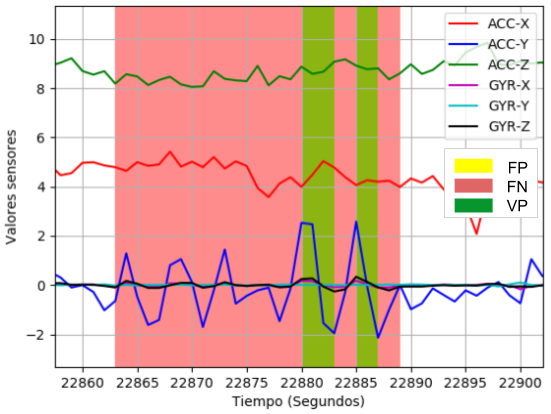
\includegraphics[width=\textwidth]{imagenes/Cap5/zig_zag1}
        \end{subfigure}       
        \begin{subfigure}[h]{0.45\textwidth} 
            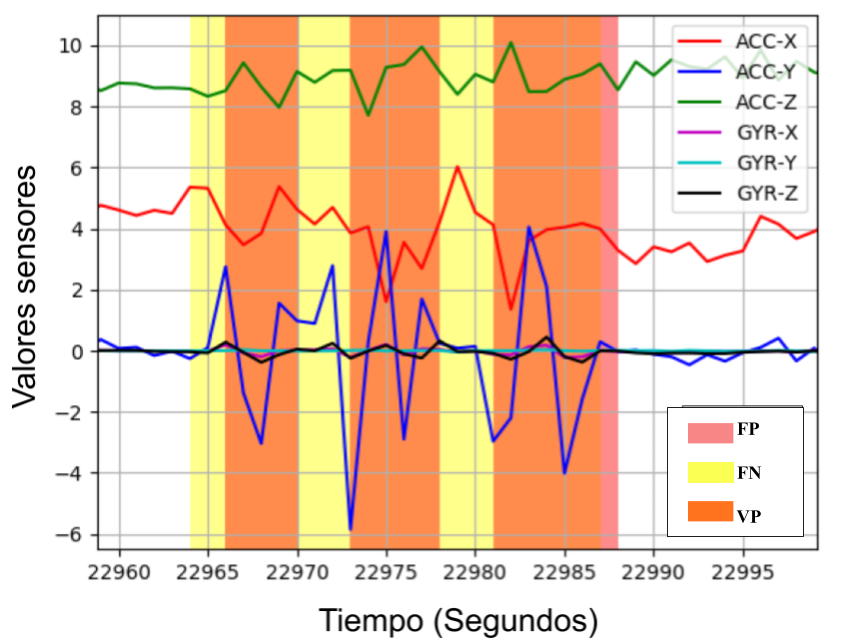
\includegraphics[width=\textwidth]{imagenes/Cap5/zig_zag2}
        \end{subfigure}
        \begin{subfigure}[h]{0.45\textwidth} 
            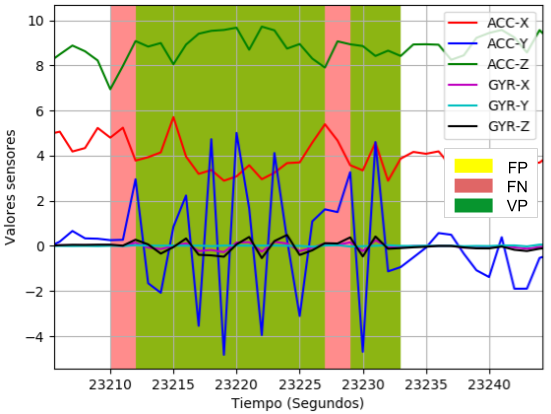
\includegraphics[width=\textwidth]{imagenes/Cap5/zig_zag3}
        \end{subfigure} 
        \end{varwidth}}
        \caption{Resultados de la detecci\'{o}n de anomal\'{i}as del tipo zig zag.}
		\label{fig:resultados_zigzag}
    \end{figure}
    
Antes de realizar el an\'{a}lisis de los resultados obtenidos se debe aclarar que aquellas secciones de las siguientes gr\'{a}ficas que se presentan en color amarillo son los valores que pertenecen al conjunto de anomal\'{i}as que no fueron correctamente detectados (Falsos negativos), las secciones en rojo corresponden a los falsos positivos y por \'{u}ltimo las secciones naranjas son los verdaderos positivos, es decir, aquellos valores que fueron detectados correctamente como anomal\'{i}as.

\vspace{5mm} %5mm vertical space

Como se observa en la Gr\'{a}fica \ref{fig:resultados_zigzag}, la imagen superior izquierda presenta una gran cantidad de falsos negativos, esto se debe a que las oscilaciones de los movimientos en Zig Zag no fueron lo suficientemente bruscos, en comparaci\'{o}n a los dem\'{a}s, por otro lado la imagen superior derecha presenta una cantidad moderada de falsos negativos y un ejemplar de falso positivo, aunque el resultado no parezca del todo bueno realmente si lo es, ya que muchos de los falsos negativos se encuentran entre valores detectados correctamente, lo cual conllevaria a una correcta generaci\'{o}n de alarma de anomal\'{i}as a pesar de no detectar como valor at\'{i}pico la totalidad de los datos an\'{o}malos, en la imagen inferior se presenta un ejemplo similar, aunque en este caso no se detectan falsos positivos.

\subsection{Detecci\'{o}n de anomal\'{i}as del tipo giros a alta velocidad}

Este tipo de anomal\'{i}as suelen ser comunes en agentes que conducen bajo los efectos del alcohol, drogas o con un estado emocional alterado, dichos datos se consideran anomal\'{i}as ya que los giros normalmente se realizan bajando la velocidad del veh\'{i}culo, y al realizar este tipo de actos un agente es propenso a ser el causante de un accidente de tr\'{a}nsito.

\vspace{5mm} %5mm vertical space

La Figura \ref{fig:resultados_giros} muestra los resultados obtenidos para las anomal\'{i}as del tipo giros a alta velocidad, las tres imagenes presentan resultados muy similares, todas tienen una secci\'{o}n en la parte inicial que se presenta como falso negativo, es decir tienen una proporci\'{o}n de datos que no son detectadas correctamente, posteriormente cuentan con un bloque de verdaderos positivos, y por \'{u}ltimo, dos de las tres imagenes cuentan con un ejemplar de falso positivo porterior a la anomal\'{i}a. A pesar de que este tipo de anomal\'{i}as no son detectadas completamente, todas presentan una secci\'{o}n que si es detectado como anomal\'{i}a, lo cual es suficiente para generar una alarma oportunamente.

\begin{figure}[H]
        \centering
        
\fbox{\begin{varwidth}{\textwidth}

        \centering
        \begin{subfigure}[h]{0.45\textwidth} 
            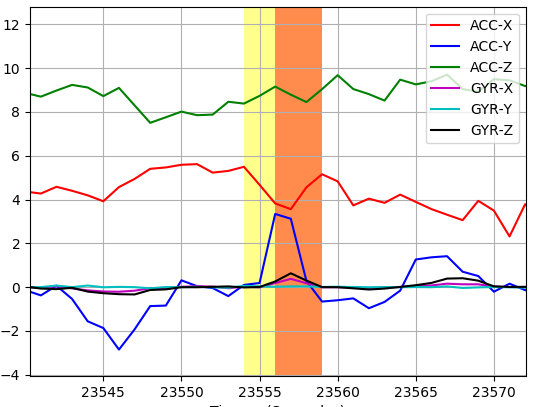
\includegraphics[width=\textwidth]{imagenes/Cap5/giro1}
        \end{subfigure}       
        \begin{subfigure}[h]{0.45\textwidth} 
            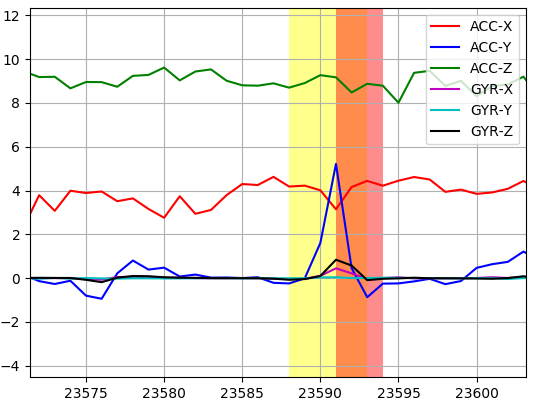
\includegraphics[width=\textwidth]{imagenes/Cap5/giro2}
        \end{subfigure}
        \begin{subfigure}[h]{0.45\textwidth} 
            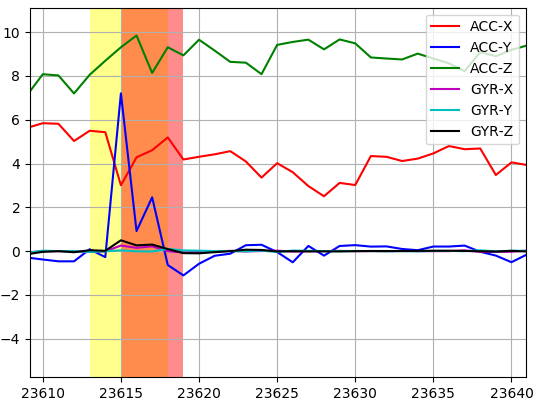
\includegraphics[width=\textwidth]{imagenes/Cap5/giro3}
        \end{subfigure} 
        \end{varwidth}}
        \caption{Resultados de la detecci\'{o}n de anomal\'{i}as del tipo giros a alta velocidad.}
		\label{fig:resultados_giros}
    \end{figure}

\subsection{Detecci\'{o}n de anomal\'{i}as del tipo frenos en seco}

Este tipo de anomal\'{i}a suele ser uno de los valores at\'{i}picos m\'{a}s comunes que existen, ya que no s\'{o}lo se presentan bajo los efectos del alcohol, drogas o fallas mec\'{a}nicas, sino que tambi\'{e}n se presentan en contextos de distracci\'{o}n del conductor ya sea por el uso del celular u otro tipo de distracci\'{o}n, ante la aparici\'{o}n de un peat\'{o}n o mascota que se presenta de manera repentina en la carril que conduce el agente, entre otros casos.

\vspace{5mm} %5mm vertical space

Los resultados de la detecci\'{o}n de este tipo de anomal\'{i}a se presentan en la Figura \ref{fig:resultados_frenos}, donde al igual que el caso anterior este tipo de anomal\'{i}a presenta una secci\'{o}n de falsos negativos, posteriormente un grupo de anomal\'{i}as correctamente detectadas y finalmente falsos positivos; con lo cual es suficiente para generar alertas de manera oportuna y de esa manera poder evitar en lo posible alg\'{u}n accidente de tr\'{a}nsito.

\begin{figure}[H]
        \centering
\fbox{\begin{varwidth}{\textwidth}

        \centering
        \begin{subfigure}[h]{0.45\textwidth} 
            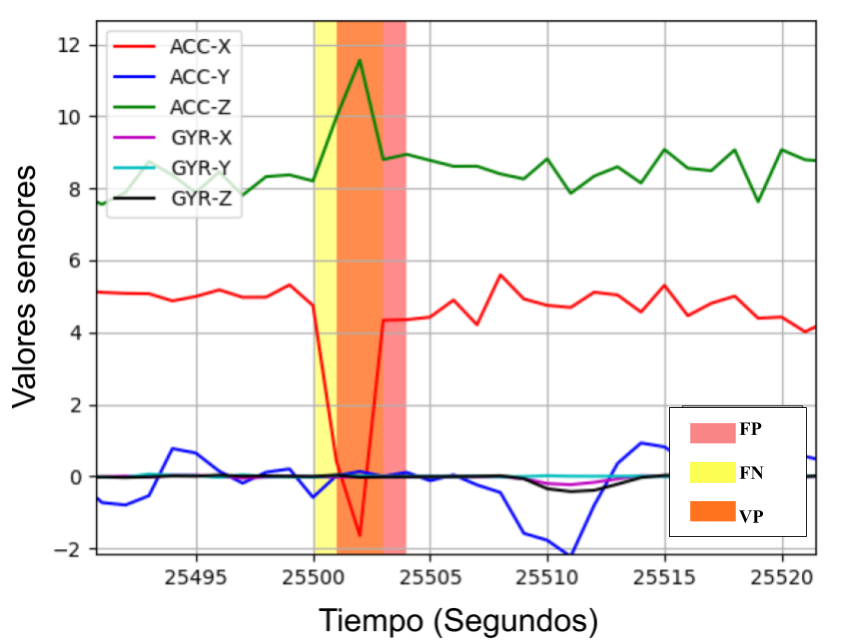
\includegraphics[width=\textwidth]{imagenes/Cap5/freno1}
        \end{subfigure}       
        \begin{subfigure}[h]{0.45\textwidth} 
            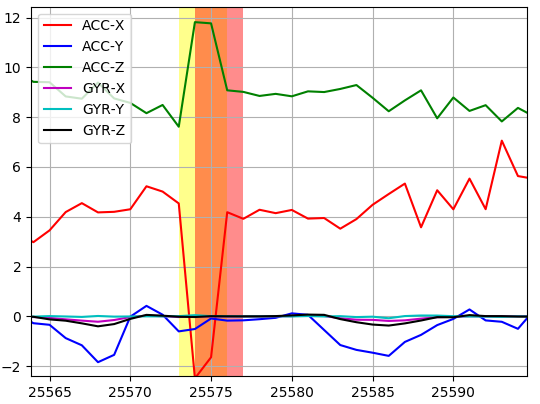
\includegraphics[width=\textwidth]{imagenes/Cap5/freno2}
        \end{subfigure}
        \begin{subfigure}[h]{0.45\textwidth} 
            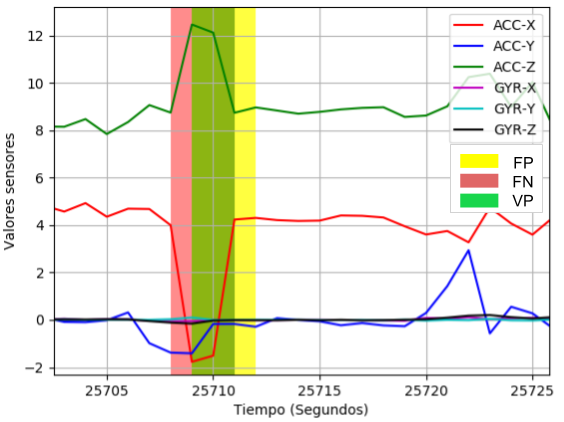
\includegraphics[width=\textwidth]{imagenes/Cap5/freno3}
        \end{subfigure} 
        \end{varwidth}}
        \caption{Resultados de la detecci\'{o}n de anomal\'{i}as del tipo frenos en seco.}
		\label{fig:resultados_frenos}
    \end{figure}


\subsection{Detecci\'{o}n de falsos positivos}

As\'{i} como se detect\'{o} una gran cantidad de anomal\'{i}as mediante este mecanismo, tambi\'{e}n se detect\'{o} una proporci\'{o}n considerable de falsos positivos, es decir, valores normales que fueron detectados err\'{o}neamente como valores at\'{i}picos.

\vspace{5mm} %5mm vertical space

De la misma forma que es importante conocer como este m\'{e}todo detecta anomal\'{i}as, tambi\'{e}n es importante saber en que casos el modelo propuesto falla; en la Figura \ref{fig:resultados_falsos_positivos} se presenta algunos casos donde el modelo falla, es decir, esta figura presenta algunos ejemplos de falsos positivos. La figura \ref{fig:resultados_falsos_positivos} ilustra claramente que estos falsos positivos se presentan generalmente de forma aislada, es decir, uno o dos valores detectados err\'{o}neamente como anomal\'{i}as de forma continua, lo cual es un comportamiento diferente al de los verdaderos valores at\'{i}picos, ya que estos presentan una detecci\'{o}n de tres valores at\'{i}picos de forma continua minimamente.

\begin{figure}[H]
        
        \centering
\fbox{\begin{varwidth}{\textwidth}

        \centering
        \begin{subfigure}[h]{0.45\textwidth} 
            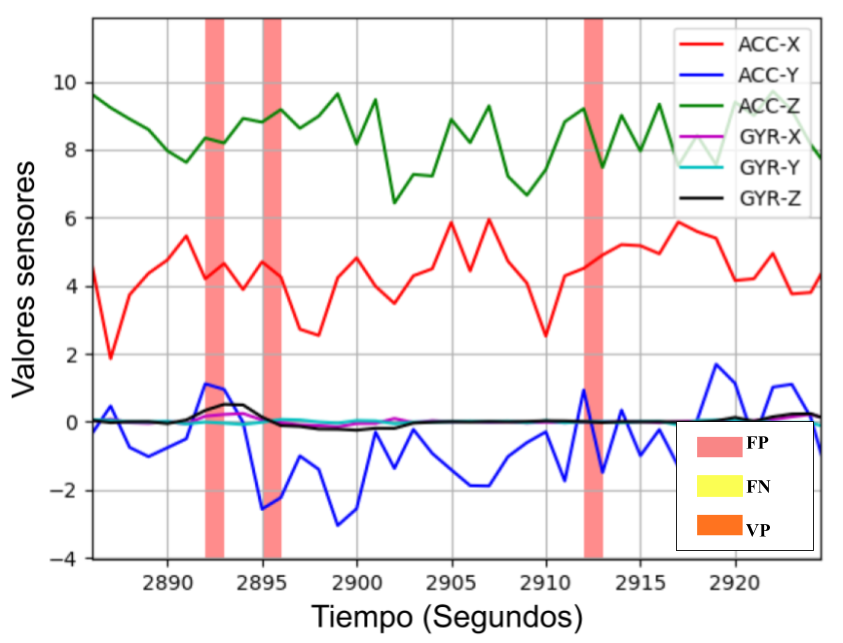
\includegraphics[width=\textwidth]{imagenes/Cap5/fp1}
        \end{subfigure}       
        \begin{subfigure}[h]{0.45\textwidth} 
            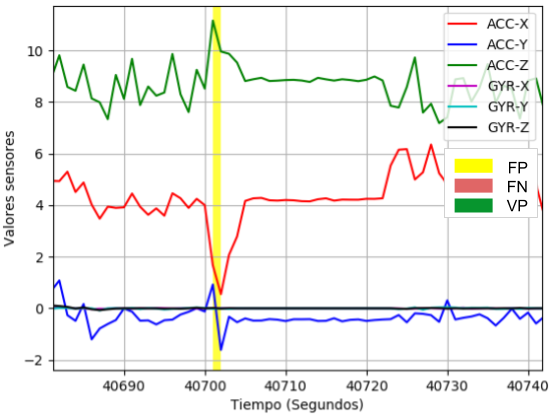
\includegraphics[width=\textwidth]{imagenes/Cap5/fp2}
        \end{subfigure}
        \begin{subfigure}[h]{0.45\textwidth} 
            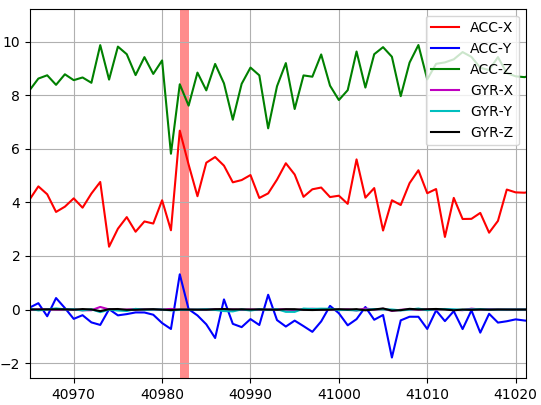
\includegraphics[width=\textwidth]{imagenes/Cap5/fp3}
        \end{subfigure} 
        \end{varwidth}}
        \caption{Resultados de la detecci\'{o}n de falsos positivos.}
		\label{fig:resultados_falsos_positivos}
    \end{figure}

\section{Resumen}

Este cap\'{i}tulo detall\'{o} el tipo de evaluaci\'{o}n al que se someti\'{o} el mecanismo propuesto en el trabajo de investigaci\'{o}n, para finalmente presentar los resultados que se obtuvieron por cada tipo de anomal\'{i}a.
 
 